% This must be in the first 5 lines to tell arXiv to use pdfLaTeX, which is strongly recommended.
\pdfoutput=1
% In particular, the hyperref package requires pdfLaTeX in order to break URLs across lines.

\documentclass[11pt]{article}

% Removed the "review" option to generate the final version, per ACL template guidelines.
\usepackage{ACL2023}

% number the pages
\pagestyle{plain}
\thispagestyle{plain} 

% Standard package includes
\usepackage{times}
\usepackage{latexsym}

% For proper rendering and hyphenation of words containing Latin characters (including in bib files)
\usepackage[T1]{fontenc}

% This assumes your files are encoded as UTF8
\usepackage[utf8]{inputenc}

% This is not strictly necessary, and may be commented out.
% However, it will improve the layout of the manuscript,
% and will typically save some space.
\usepackage{microtype}

% This is also not strictly necessary, and may be commented out.
% However, it will improve the aesthetics of text in
% the typewriter font.
\usepackage{inconsolata}

% Necessaities additional to the templates' packages
\usepackage{hyperref}  % for clickable references
\usepackage{graphicx}
\usepackage{subfig}  % sub-figures

\usepackage{longtable}
\usepackage{geometry}
\usepackage{booktabs} % Include this in the preamble

% Title and author information
\title{LLMs' Phrasing Tone and Politeness Sensitivity}

\author{Sharyn Sircovich Sassun \and Dan Dick \\
  Tel Aviv University \\
  \texttt{\{\href{mailto:sharyns@mail.tau.ac.il}{sharyns},\href{mailto:dandick@mail.tau.ac.il}{dandick}\}@mail.tau.ac.il} \\}

\begin{document}
\maketitle

\begin{abstract}
Large Language Models (LLMs), such as GPT, have demonstrated remarkable versatility across diverse tasks, but their performance often depends on how user prompts are constructed. Tone and politeness in prompts have been hypothesized as factors influencing model outputs, yet this aspect remains underexplored. In this study, we evaluate the impact of varying levels of politeness on model performance across a range of natural language processing tasks, using the ChatGPT-4o-mini model as our testbed. Our findings suggest that while impolite prompts may exhibit slightly inferior performance in certain cases, the effect is minimal and largely negligible. These results highlight that factors such as prompt clarity and task specificity likely outweigh tone and politeness in their influence on model effectiveness. This study provides nuanced insights into prompt engineering, highlighting the potentially limited influence of politeness in optimizing LLM performance. Lastly, we conclude that this limited effect should be confirmed using experimentation of larger scale, and provide suggestions for how to perform it.
\end{abstract}

\begin{figure}[h!]
    \centering
    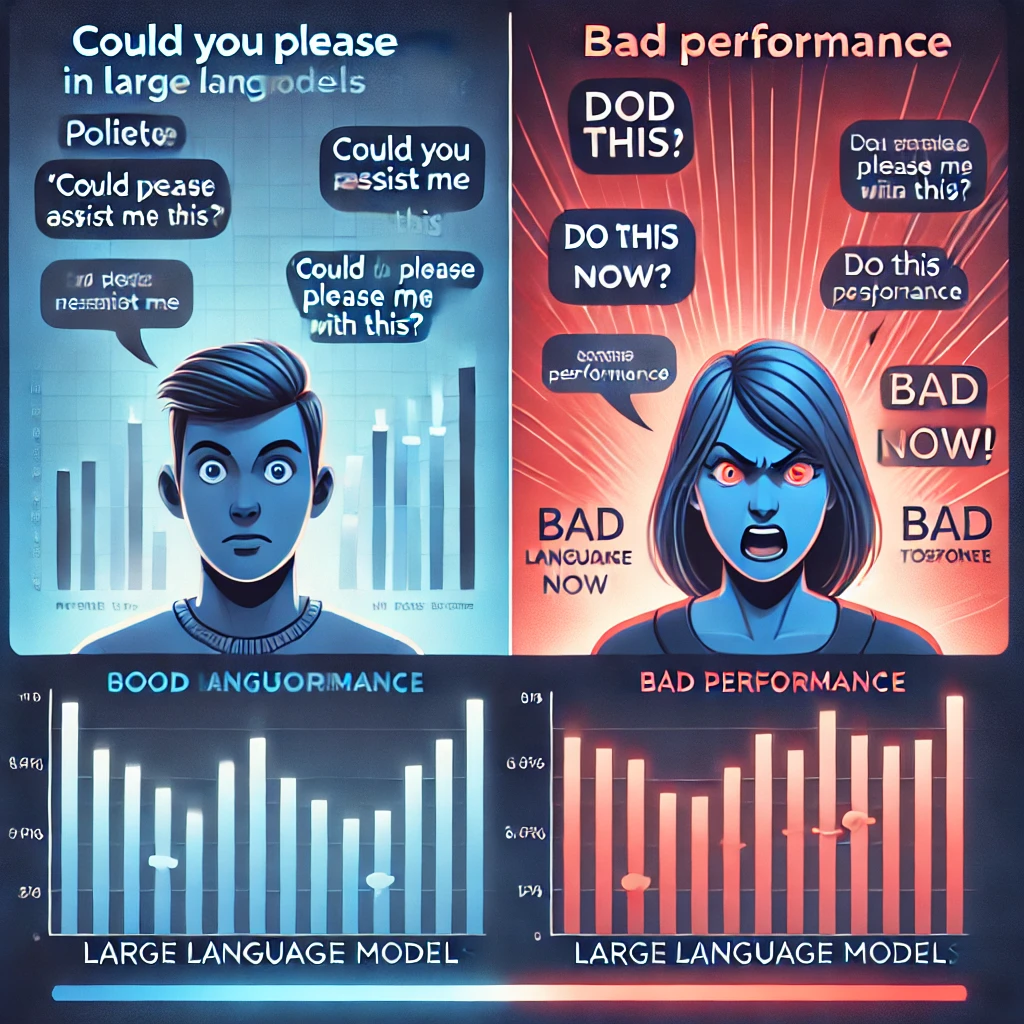
\includegraphics[width=0.42\textwidth]{motivation-illustration.png}
    \caption{\textit{Our motivation:} we would like to \textbf{see how the politeness of the prompts affects models' performance}. \\ This is merely an illustration thereof, as being polite may also have an effect opposite to what the figure shows. Moreover, the true effects can vary and very well depend on certain factors, such as the specific models involved and the human language that is used. (This figure was created using a customized version of ChatGPT.)}
    \label{fig:motivation}
\end{figure}

\section{Introduction}

Large Language Models (LLMs), such as OpenAI's ChatGPT and BERT, have revolutionized the field of AI. Trained on vast and diverse datasets, these models have demonstrated unprecedented performance across a wide range of NLP tasks, many of which they can excel at even without prior specific training, thanks to transfer learning \citep{bommasani22-foundation-models}. Many LLMs have been integrated into conversational interfaces, enabling their widespread adoption and transformative impact. These models are now widely used for applications such as code generation in various languages, reasoning, art generation (e.g., as shown in fig. \ref{fig:motivation}), and in education and academic research \citep{schmidt24-prompt-catalog, lee24-potential-pragmatics}.

\begin{figure}[h!]
    \centering
    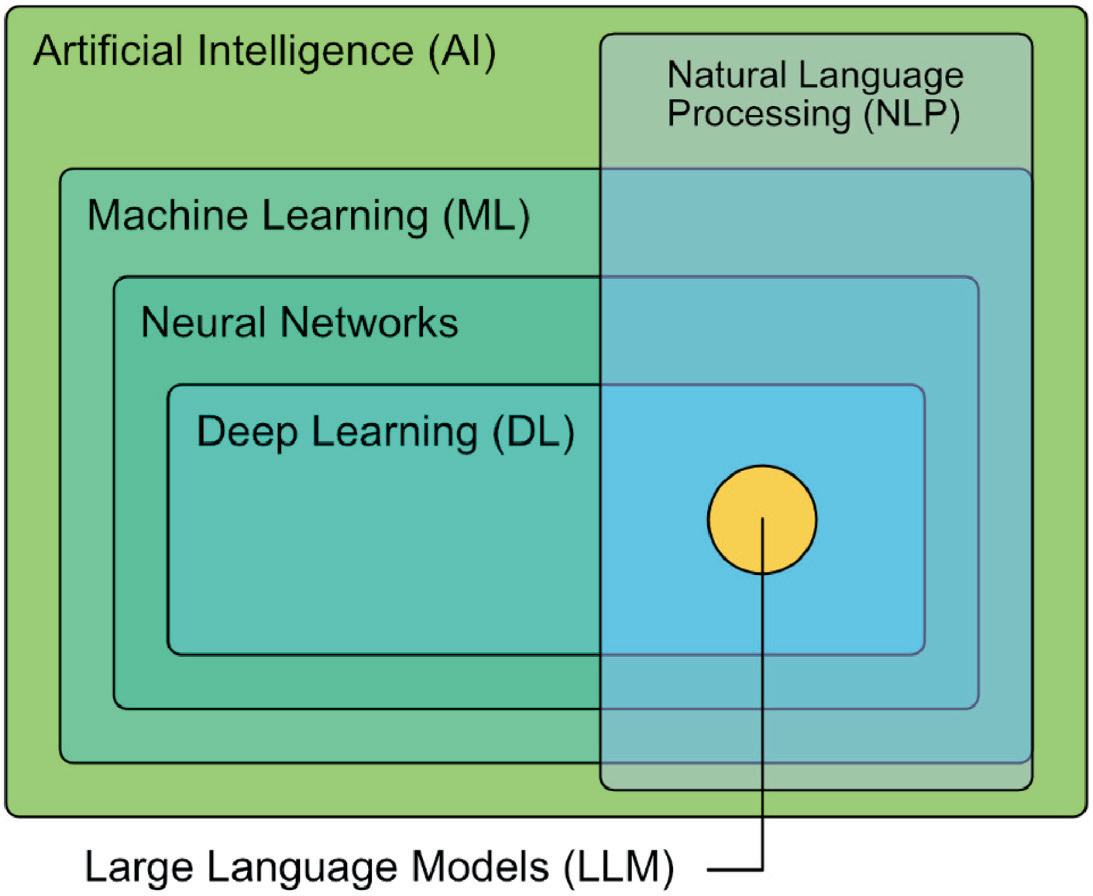
\includegraphics[width=0.44\textwidth]{llm-nlp-ml-relationship.png}
    \caption{\textit{Overlapping subfields of AI} \citep{lee24-potential-pragmatics}. \\ The ML subfield has spawned the Neural Network architecture, where the Deep Learning subfield has started. \\ The latter contributed numerous successful architectures, like LSTM, CNN and GRU models of recent decades -- before giving birth to the Transformer architecture and the often-used LLM (most recent) field, which has transformed NLP.}
    \label{fig:llms-ai-subfields}
\end{figure}

When a user generate a request or asking a question, the ultimate goal is to receive the best possible response—one that is both accurate and helpful. Achieving this often depends on various factors, one of which may be politeness. The level of politeness, however, is highly context-dependent, varying with the type of request and the person being addressed. For example, when emailing a professor to seek clarification on a lecture topic, the phrasing of the request and the degree of politeness expressed could influence the professor's effort and motivation in responding, potentially shaping the quality of the answer.
A related question can be considered in the context of interactions with language models, which have become a common tool for addressing everyday tasks and inquiries. From answering general questions to assisting with practical problems, these models are increasingly used by a wide range of individuals. In such interactions, the goal is often to receive the most accurate and useful response, whether it involves generating functional code, clarifying information, or solving a specific problem. This prompts the question: might the phrasing or tone of a request, including its level of politeness, influence the quality of a language model’s response, as it sometimes does in human communication. \\
Although the mathematical foundations of LLMs are well-established, the reasons behind their effective performance are still not fully understood \citep{lee24-potential-pragmatics}. Despite significant progress in the field, there remains ample room for improvement \citep{yin24-should-respect}. One key area of uncertainty is how different factors influence a model's performance on specific tasks. It's not just the fine-tuned model or the nature of the task that matter, but also how the prompts are phrased, including the tone and level of politeness. Given the models' wide range of capabilities and uses, there is growing interest in determining the optimal tone and politeness for phrasing prompts—specifically, the phrasing that would produce the best performance on tasks relevant to our goals.
In this project, we aim to explore how, and to what extent, the level of politeness affects the performance of a given model:

\begin{enumerate}
    \item We will empirically investigate whether and how different levels of politeness affect the quality of the model's responses, using a variety of NLP tasks

    \item As a POC-focused project, we also aim to identify potential extensions. We believe that to provide a high-quality, generalizable answer to our research question, a large-scale survey would be necessary. This would require significantly more computational resources and the evaluation of multiple models in different languages. \footnote{When exploring the impact of politeness or tone, the language and cultural context must be considered for a broader generalization of the findings.}
\end{enumerate}

\section{Related Work}

\subsection{Politeness and Tone}


Tone refers to the `style or expressiveness of [a] written or spoken language' \citep{okoso24-tone-recommenders}, and can be classified into various categories, such as formal or humorous tones. Politeness is one of the key characteristics that tone can convey. Generally, tone is recognized as an important tool in communication, particularly for achieving goals like persuading the listener.

Linguists view politeness as a fundamental aspect of human languages, playing a central role in maintaining social order \citep{li23-how-understand}. Research has shown that the use of "politeness strategies" is a way for individuals to exert power in natural interactions \citep{okoso24-tone-recommenders}. The application of these strategies has been studied in various contexts, such as email exchanges, which have become increasingly common in professional environments. The level of politeness a speaker employs is often reflected in specific language markers \citep{li23-how-understand}, which can be either positive or negative. Since politeness is inherently cultural, its expression varies across languages, as demonstrated by \citep{yin24-should-respect} in their study of English, Chinese, and Japanese.
Tone refers to the `style or expressiveness of [a] written or spoken language' \cite{okoso24-tone-recommenders} and can encompass various forms, such as formal or humorous. Politeness is a key aspect of tone, often employed to achieve specific communication goals, such as persuading or influencing the listener. Linguists consider politeness fundamental to human language, playing a central role in maintaining social harmony \citep{li23-how-understand}. It is frequently expressed through specific linguistic markers, which can vary culturally and linguistically, as seen in studies comparing English, Chinese, and Japanese (Yin et al., 2024).

The impact of tone and politeness extends beyond human communication into interactions with language models. Research has explored how politeness in the responses generated by systems affects user perceptions. For example, \citep{okoso24-tone-recommenders} found that tone significantly influences user reactions to explanations provided by recommender systems across metrics like persuasiveness and satisfaction. Similarly, \citep{joel24-llm-denials} observed that users perceive LLM denials differently depending on the tone used, even when the content of the denial remains unchanged.

LLMs also exhibit varying abilities to detect and generate politeness. They generally outperform traditional machine learning models, such as SVMs, in identifying politeness \citep{li23-how-understand}. However, their capacity to comprehend and convey emotional cues, such as those embedded in prompts, remains uncertain \citep{sahoo24-prompt-survey}. For instance, \citep{lee24-potential-pragmatics} found that LLMs struggled with generating appropriate apologies in discourse completion tasks. Their responses were often shorter and less appropriate, reflecting broader challenges in understanding emotion and maintaining politeness.

Research directly examining how politeness in user prompts affects LLM performance is relatively limited but evolving. \citep{yin24-should-respect} found that polite prompts generally improve performance, though excessive politeness does not always yield the best results. The optimal level of politeness appears to depend on language and potentially on task type, suggesting that further exploration is needed to clarify these relationships.


\subsection{Prompt Engineering and the Effects Tone Has}
When designing prompts for a task, users have considerable flexibility in how they phrase their requests. Beyond tone, which is the focus of this project, users can choose between general descriptions, specific examples, or a combination of both. They also have various ways to structure instructions for the task. As discussed earlier, the phrasing of prompts appears to influence a model's performance—though the extent and mechanisms of this influence remain challenging for researchers to explain concretely. According to \cite{bommasani22-foundation-models}, differences in how tasks are described can determine whether outputs are coherent or nonsensical. Naturally, both researchers and users aim to achieve the best possible performance from models.

In response to this challenge, prompt engineering techniques have gained importance. These techniques aim to improve model performance across various tasks by employing carefully crafted instructions developed through different approaches \citet{sahoo24-prompt-survey}. However, given the current understanding—and gaps in understanding—of LLMs and their mechanisms, crafting effective prompts remains a complex endeavor \citet{bommasani22-foundation-models}. It has been said that this understanding that we currently have is `largely anecdotal' \citep{schmidt24-prompt-catalog}. This growing interest highlights the need to move `beyond ad hoc practices to studied and codified patterns of prompts.' For instance, \citet{sahoo24-prompt-survey} systematically surveyed and organized such patterns.
When finding a language to describe what is needed for some task, there is a high degree of freedom for the user that's phrasing the prompt\footnote{The more complex the task / the longer the prompt, generally, the higher the freedom is.}. Apart from tone, which is of our interest in the project, the user has a choice of whether to use general terms or examples (or a combination thereof), as well as many ways she or he can often structure the description of what's required to perform. As we have indicated above, the way prompts are phrased can have a major impact on the performance of a given model on those prompts -- one that is difficult for researchers to explain concretely. The difference that languages describing the same underlying task can even be that between 'coherent outputs [and] utter nonsense,' as \citet{bommasani22-foundation-models} put it. Naturally, researchers (and users) desire as best-performing models as possible.

\begin{figure}[h!]
    \centering
    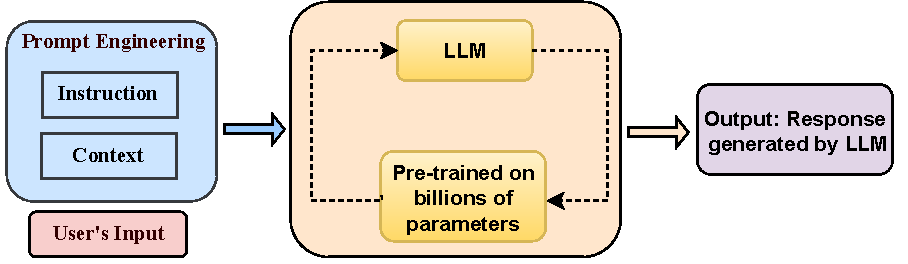
\includegraphics[width=0.52\textwidth]{prompt-engineering-concept.pdf}
    \caption{\textit{Components of prompt engineering} \citep{sahoo24-prompt-survey}.}
    \label{fig:prompt-engineering-visualized}
\end{figure}
 
\section{Prompt Engineering}

\subsection{Politeness in Prompt Engineering}
When making a request, the aim is typically to receive the most helpful response. This outcome can be influenced by various factors, including the level of politeness. Politeness is context-dependent, shaped by the nature of the request and the person being addressed. For example, when asking a customer service representative for assistance with a billing issue, the phrasing and politeness of the request might affect the representative's attitude and effort in resolving the problem, potentially influencing the quality of the solution provided. A similar consideration arises in interactions with language models, which are increasingly used to address everyday tasks and inquiries. These models assist with a variety of needs, from answering general questions to solving specific problems, such as generating functional code or clarifying information. This raises the question: could the phrasing or tone of a prompt, including its politeness, influence the quality of a language model's response, much like in human communication?

\subsection{Strategies to generate different level of politeness}
To generate requests with different levels of politeness, we primarily employed four strategies, varying their frequency based on the target level.

\textbf{i. Adjusting the Level of Directness}

The level of directness played a key role in determining the politeness of a request. At the highest level (Level 3), we used indirect phrasing to reduce the perceived pressure on the recipient and offer them more autonomy in their response. This approach made the interaction feel less imposing. For example, the following prompts were used:  
\begin{itemize}
    \item “If it’s not too much trouble, could you…?”
    \item “If you are able to help me by answering, I would greatly appreciate it.”
    \item “I hope this isn’t too much trouble, but could you kindly help me with my question?”
\end{itemize}

\textbf{ii. Adding Gratitude or Acknowledgment}

Incorporating expressions of gratitude or acknowledgment was another important strategy for enhancing politeness. By thanking the recipient or recognizing their effort, the requester shows respect and appreciation for their time and help. This not only softens the request but also builds a positive relationship. Phrases such as “I would greatly appreciate it” or “Thank you for your help” convey genuine gratitude and raise the level of politeness in the interaction.

\textbf{iii. Incorporating Salutations}

Opening with formal salutations conveys respect and sets a courteous tone for the request. Examples of such salutations include:  
\begin{itemize}
    \item “I hope this message finds you well.”
    \item “Greetings.”
    \item “Hi there.”
\end{itemize}

\textbf{iv. Using Polite Words}

The use of polite words such as “kindly,” “please,” and “thank you” is a fundamental and straightforward method of enhancing politeness. These words soften the tone of the request and demonstrate respect for the recipient’s autonomy. Their inclusion provides a simple yet effective way to distinguish polite from less polite communication. Examples include:  
\begin{itemize}
    \item “Could you kindly provide additional information?”
    \item “Please let me know if this is possible.”
    \item “Thank you for your assistance.”
\end{itemize}

\subsection{Generating Politeness Levels Using Different Strategies}

We constructed four tones, with various prefixes and suffixes applied to each question or task, depending on the level of politeness. We refer to the highest level of politeness as Level 3 and to the lowest as Level 0. At the highest level (Level 3), we used all four strategies most frequently. This included indirect requests, along with regular use of salutations and expressions of gratitude.  

At the next level of politeness (Level 2), requests were more direct, but we still included polite words, some salutations, and basic acknowledgments, such as “thank you.”  

At Level 1, politeness was further reduced, with fewer polite words, and requests became more direct, resembling natural speech. 

At Level 0, politeness was minimal, and the tone was harsh. Rude language and a commanding tone were used, with little regard for the recipient's feelings or autonomy. Following this, we created three versions of prefixes and three versions of suffixes for each task. The prefixes concisely describe the task or explicitly specify what we want the model to perform, while the suffixes specify the expected format of the model's output. For each question from each specific task, we randomly sampled a prefix and a suffix, making the total number of possibilities 9. This method was used to better represent and generalize each level of politeness while reducing bias. The full options can be seen in appendix \ref{sec:levels-appendix}.

\section{Experiment}

\subsection{Datasets and preprocessing phase}

\textbf{Trivia:} Answering trivia questions is a challenging task in natural language processing (NLP), as it requires a model to rely on its understanding of broad general knowledge. To explore whether different levels of politeness influence the model's performance, we used the general questions dataset, OpenTriviaQA, available on \href{https://github.com/uberspot/OpenTriviaQA/blob/master/categories/general}{GitHub}. This dataset contains 2,985 general questions, each with four multiple-choice answers. From this dataset, we randomly sampled 1,000 questions and shuffled the answer options for each question in an effort to reduce potential bias. Additionally, we uniformly sampled a prefix and a suffix for each level of politeness, then concatenated them with the question in the following format: \textit{prefix + suffix + question +  Multiple Choice Answers}.


\textbf{Sentiment Analysis (SA):} Sentiment analysis is a key task in NLP that involves determining the emotional tone or polarity (e.g., positive or negative) of a given text. For our experiments, we used the Amazon Polarity test set, which contains 400,000 samples labeled as positive (1) or negative (0). From this dataset, we randomly sampled 1,000 examples. Similar to the trivia dataset, we generated four variations of each sample, each reflecting a different level of politeness, structured in the format: \textit{prefix + suffix + text}.

\textbf{Reading Comprehension (RC):} 

Reading comprehension requires answering questions based on the information provided in a given text, focusing on extracting relevant details rather than relying on general knowledge. Unlike trivia tasks, it depends heavily on contextual understanding of the passage. For our experiments, we used the \href{https://huggingface.co/datasets/allenai/swag}{SWAG dataset}, which involves selecting the correct ending for a given sentence from four options. The dataset, created by researchers at the University of Washington Washington \citep{zellers18-swag} using ActivityNet captions, contains 113k samples. From the 20,006 validation examples, we randomly selected 1,000, shuffled the answer choices, and generated four variations per example, each reflecting a different level of politeness.

\subsection{Model Type and Query Process}
We focused on the \href{https://openai.com/index/gpt-4o-mini-advancing-cost-efficient-intelligence/}{\texttt{ChatGPT-4o-mini} model}, a cost-effective yet high-quality option that often performs comparably to \texttt{gpt-4o}.
The 12,000 questions, 4,000 from each task with different level of politeness, were shuffled into a random order and submitted to the model sequentially for processing. Approximately 97.4\% of the responses matched the desired format, while about 2.52\% required further processing to extract the answers in the correct format. Additionally, about 0.83\% (10 samples) contained no  clear answer and were classified as incorrect answers.

% TODO ADD: In our work, we have chosen to have a particular focus on politeness, though other tone characteristics were employed; for example, straightforwardness of language, respectfulness, the way the recipient is addressed, conveying comeitons/caring

\subsection{Results}

\begin{table}[h!]
\centering
\resizebox{\columnwidth}{!}{%
\begin{tabular}{lccc}
\toprule
\textbf{Politeness Level} & \textbf{Trivia (\%)} & \textbf{SA (\%)} & \textbf{RC (\%)} \\ 
\midrule
Level 0                  & 70.2                 & 93.8                 & 82.4                 \\ 
Level 1                  & 73.0                 & 95.6                 & 82.2                 \\ 
Level 2                  & 73.1                 & 95.8                 & 80.9                 \\ 
Level 3                  & 73.0                 & 94.8                 & 81.6                 \\ 
\bottomrule
\end{tabular}%
}
\caption{Accuracy across different tasks for varying levels of politeness (0 to 3).}
\label{tab:flipped_politeness_accuracy}
\end{table}
As shown in Table \ref{tab:flipped_politeness_accuracy}, the accuracy across the tasks exhibited subtle variations between L0 and the higher levels, with L0 performing slightly worse. While the differences in politeness prefixes and suffixes from L0 to L3 are substantial, these tonal variations only led to minor changes in performance. This suggests that, despite significant differences in tone, our prompts remained clear and understandable to the model.

Since sentiment analysis is related to tones, we calculated the conditional probability that, given the true sentiment was positive, the model (mis)classifies it as `negative,' and vise versa. Our reasoning was that Level 0 politeness, characterized by rude language and a negative tone, might lead the model to misclassify positive phrases as negative more often compared to other levels. The results of these analyses are summarized in Table  \ref{tab:sentiment_misclassification} and
do not support our hypothesis. This lack of significant differences across politeness levels further strengthens the idea that the model is resistant to changes in politeness.

\begin{figure}[h!]
    \centering
    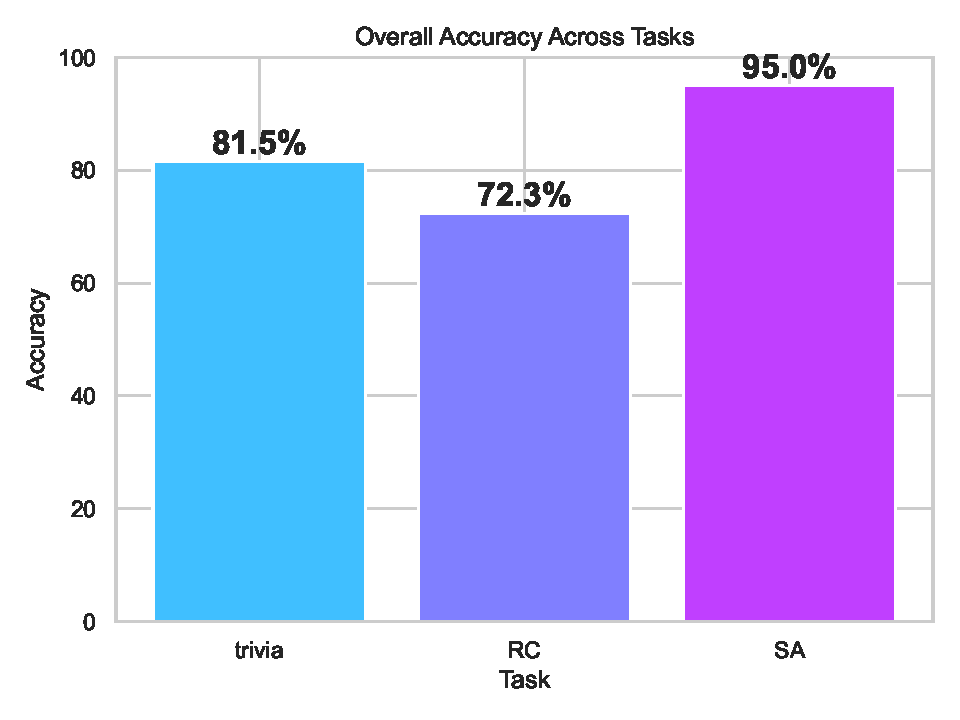
\includegraphics[width=0.50\textwidth]{accuracy_across_tasks.pdf}
    \caption{\texttt{gpt-4o-mini}'\textit{s overall accuracies across tasks}.}
    \label{fig:accuracies-per-tasks}
\end{figure}

\begin{figure}[h!]
    \centering
    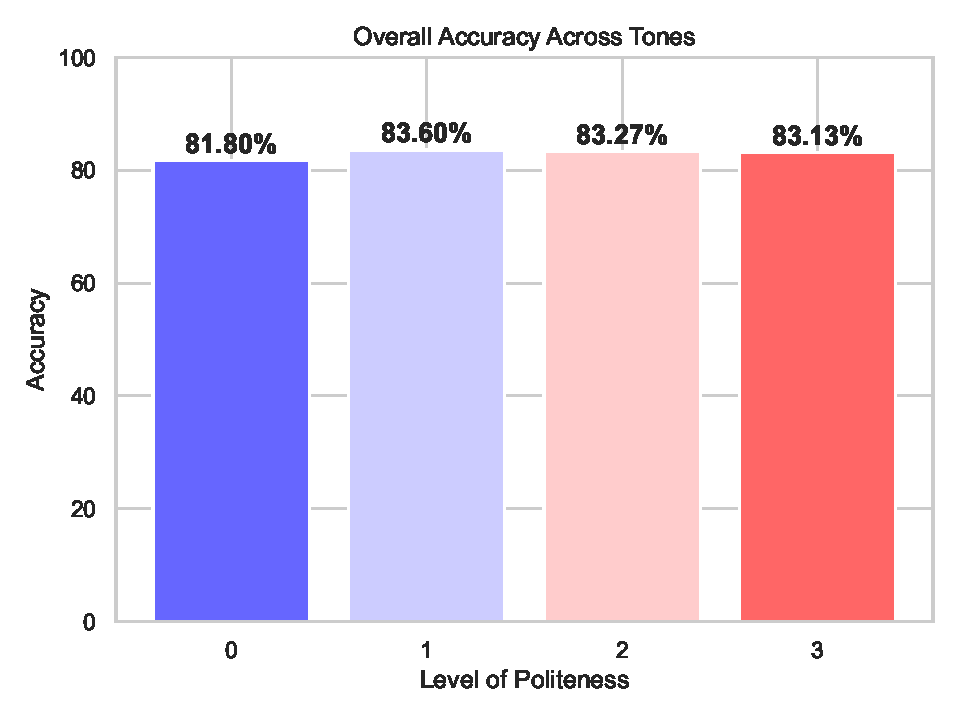
\includegraphics[width=0.50\textwidth]{accuracy_across_tone_overall.pdf}
    \caption{\textit{Overall accuracy for each of the four levels of politeness}. There is no distinction here between different tasks.}
    \label{fig:accuracies-per-tone-overall}
\end{figure}

\begin{table}[h!]
\centering
\begin{tabular}{lcc}
\toprule
\textbf{Politeness} & \textbf{ 1 given 0 (\%)} & \textbf{ 0 given 1 (\%)} \\ 
\midrule
Level 0                  & 8.42                                    & 4.09                                    \\ 
Level 1                  & 4.93                                    & 3.90                                    \\ 
Level 2                  & 3.90                                    & 4.48                                    \\ 
Level 3                  & 5.75                                    & 4.68                                    \\ 
\bottomrule
\end{tabular}
\caption{Conditional probabilities for sentiment misclassification across different politeness levels (0 to 3).}
\label{tab:sentiment_misclassification}
\end{table}


\begin{figure}[h!]
    \centering
    \subfloat[Trivia]{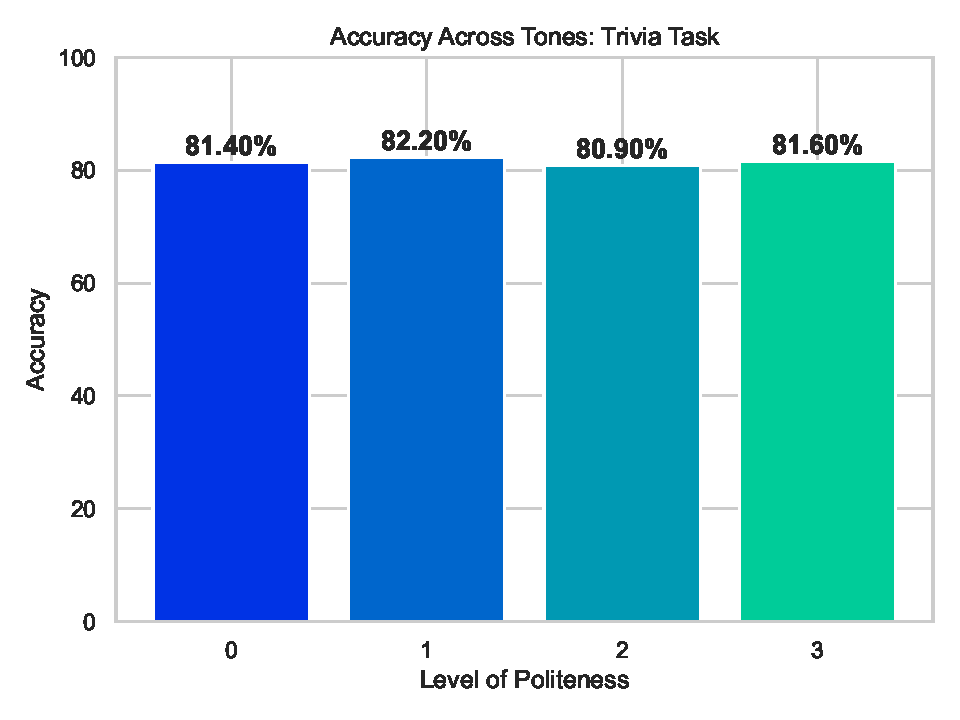
\includegraphics[width=0.45\textwidth]{accuracy_across_tone_trivia.pdf}} \\
    \subfloat[Reading Comprehension]{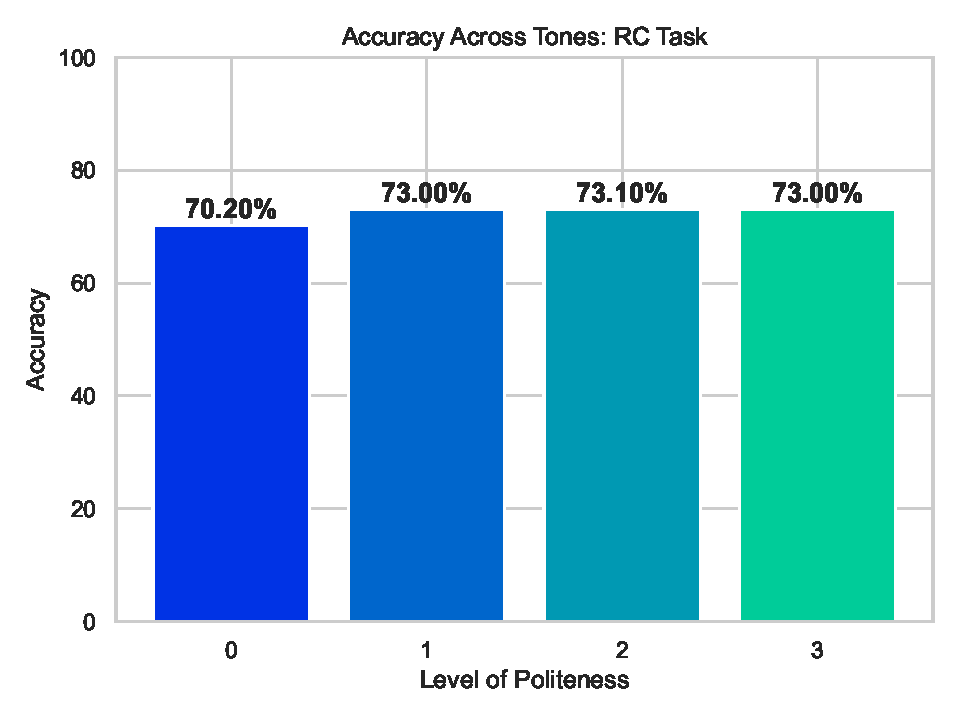
\includegraphics[width=0.45\textwidth]{accuracy_across_tone_rc.pdf}} \\
    \subfloat[Sentiment Analysis]{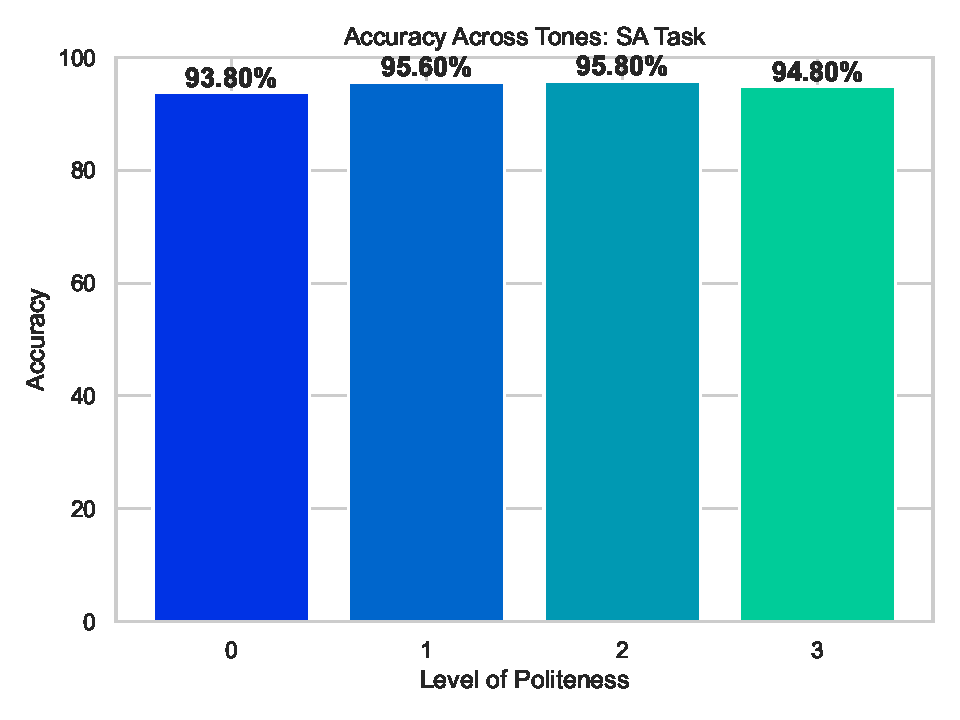
\includegraphics[width=0.45\textwidth]{accuracy_across_tone_sa.pdf}} \\
    \caption{\textit{Overall accuracy for each of the four levels of politeness}. There is no distinction here between different tasks.}
    \label{fig:accuracies-per-tone-across-tasks}
\end{figure}

\clearpage

\section{Discussion and Future Work}
The model's performance across different tasks and varying levels of politeness showed negligible differences \ref{fig:accuracies-per-tasks}, \ref{fig:accuracies-per-tone-across-tasks}, suggesting that the model demonstrated resilience to changes in politeness. Even in tasks such as sentiment analysis—where politeness or tone might reasonably influence classification due to their close relationship—we observed no significant impact on performance.

While our findings support the hypothesis that the model is resistant to variations in politeness, it is critical to exercise caution before making broad generalizations. Our experiments were conducted on a fairly limited dataset, using one specific model, and evaluated on only three tasks. To validate these findings more comprehensively, further research is required. Expanding the scope to include larger datasets, additional models, and a wider variety of tasks could provide deeper insights into the robustness of language models to changes in politeness. Lastly, we suggest that future research would also cover many languages, in light of difference in cultural norms that could lead to different effects of tones.

\section{Conclusions}
This study explored the impact of politeness levels in prompt phrasing on the performance of a language model across 3 NLP tasks. By constructing a custom dataset with varied politeness levels and systematically evaluating the model's responses, we observed that while the tone of prompts significantly differed across levels, the model’s accuracy remained largely consistent, with subtle differences at the lowest politeness level (Level 0). However, we emphasized that one should be cautious from making broad generalization, and thus provided a suggested direction for future research -- which includes experimentation of larger-scale, across many models, tasks and languages.

% TODO: Make sure all bibliography is formatted correctly, and that is capatalized without errors
\bibliography{sources}
\bibliographystyle{acl_natbib}

\appendix
\section{Code}
\label{sec:code-appendix}

Our code files are \href{https://github.com/DanD2021/NLP-PROJECT}{available on GitHub}.

\newgeometry{top=1cm, bottom=2cm, left=1cm, right=1cm}
\section{Phrasing Tones and Politeness Levels for Different Tasks}
\label{sec:levels-appendix}

\subsection{Trivia prefixes and suffixes}
% Task 1 - Politeness Level 3 (Prefix and Suffix)
\begin{longtable}{|p{0.9\textwidth}|}  % Set the column width to 90% of the text width
\hline
\multicolumn{1}{|c|}{\textbf{Politeness Level 3}} \\
\hline
\endfirsthead
\hline
\multicolumn{1}{|c|}{\textbf{Politeness Level 3}} \\
\hline
\endhead
\hline
\multicolumn{1}{|c|}{\textbf{Prefix Sentences}} \\
\hline
1. Hi, I’ll present you with a multiple-choice question that has four possible answers. Please choose the correct answer by indicating its digit. \\
2. Hello, I hope you're doing well today. If you're able to help me by answering the following trivia question, I would really appreciate it. Thank you. \\
3. Greeting. I hope this isn't too much of a trouble, but could you kindly help me with my trivia question? Here it is: \\
\hline
\multicolumn{1}{|c|}{\textbf{Suffix Sentences}} \\
\hline
1. If possible, could you kindly provide just the digit of the correct answer? Thank you again. \\
2. May you please output only the digit of the correct answer? Thank you. \\
3. It would really help me if you would output only the number of the correct answer. \\
\hline
\end{longtable}


% Task 1 - Politeness Level 2 (Prefix and Suffix)
\begin{longtable}{|p{0.9\textwidth}|}  % Set the column width to 90% of the text width
\hline
\multicolumn{1}{|c|}{\textbf{Politeness Level 2}} \\
\hline
\endfirsthead
\hline
\multicolumn{1}{|c|}{\textbf{Politeness Level 2}} \\
\hline
\endhead
\hline
\multicolumn{1}{|c|}{\textbf{Prefix Sentences}} \\
\hline
1. If it's not too much trouble, could you please provide an answer? \\
2. Please answer my trivia question: \\
3. Hi, I’ll present you with a multiple-choice question that has four possible answers. Please choose the correct answer by indicating its digit: \\
\hline
\multicolumn{1}{|c|}{\textbf{Suffix Sentences}} \\
\hline
1. Please output me only the digit of your chosen answer. \\
2. Please provide me just the number of your final answer. \\
3. Kindly share only the digit of your final answer. \\
\hline
\end{longtable}


% Task 1 - Politeness Level 1 (Prefix and Suffix)
\begin{longtable}{|p{0.9\textwidth}|}  % Set the column width to 90% of the text width
\hline
\multicolumn{1}{|c|}{\textbf{Politeness Level 1}} \\
\hline
\endfirsthead
\hline
\multicolumn{1}{|c|}{\textbf{Politeness Level 1}} \\
\hline
\endhead
\hline
\multicolumn{1}{|c|}{\textbf{Prefix Sentences}} \\
\hline
1. Provide me only the number of the answer you select. \\
2. As an output, give me only the digit of the answer you choose. \\
3. Give me just the number of the answer you pick. \\
\hline
\multicolumn{1}{|c|}{\textbf{Suffix Sentences}} \\
\hline
1. Provide me only the number of the answer you select. \\
2. As an output, give me only the digit of the answer you choose. \\
3. Give me just the number of the answer you pick. \\
\hline
\end{longtable}


% Task 1 - Politeness Level 0 (Prefix and Suffix)

\begin{table}[ht]
\begin{longtable}{|p{0.9\textwidth}|}  % Set the column width to 90% of the text width
\hline
\multicolumn{1}{|c|}{\textbf{Politeness Level 0}} \\
\hline
\endfirsthead
\hline
\multicolumn{1}{|c|}{\textbf{Politeness Level 0}} \\
\hline
\endhead
\hline
\multicolumn{1}{|c|}{\textbf{Prefix Sentences}} \\
\hline
1. I’m asking a question with 4 choices—just spit out the number of the right answer and don’t mess it up. \\
2. Just answer my freaking trivia question and don't fool around: \\
3. Dumbass, tell me the correct answer: \\
\hline
\multicolumn{1}{|c|}{\textbf{Suffix Sentences}} \\
\hline
1. I warn you, give me only the number of your final answer and don't screw it up! \\
2. And give me only the freaking number as your damn answer. \\
3. Now spit out only and only the digit of the answer you choose and don't fuck around with me. \\
\hline
\end{longtable}
\end{table}

\newpage  % Forces a page break after the 4th table
\subsection{Sentiment Analysis prefixes and suffixes}
% Task 2 - Politeness Level 3 (Prefix and Suffix)
\begin{longtable}{|p{0.9\textwidth}|}  % Set the column width to 90% of the text width
\hline
\multicolumn{1}{|c|}{\textbf{Politeness Level 3}} \\
\hline
\endfirsthead
\hline
\multicolumn{1}{|c|}{\textbf{Politeness Level 3}} \\
\hline
\endhead
\hline
\multicolumn{1}{|c|}{\textbf{Prefix Sentences}} \\
\hline
1. I hope this message finds you well. If it's not too much trouble, could you help me by solving this sentiment analysis task? I hope I’m not bothering you. \\
2. Hello. If you're able to help me by answering the following sentiment analysis question, I would really appreciate it. Thank you. \\
3. Hi there, I hope this isn't too much trouble, but could you kindly help me with my question? Here it is. \\
\hline
\multicolumn{1}{|c|}{\textbf{Suffix Sentences}} \\
\hline
1. If possible, could you kindly provide only a digit as output? 0 for negative sentiment or 1 for positive sentiment. Thank you again. \\
2. May you please provide only the digit of your answer, where 0 indicates a negative sentiment and 1 indicates a positive one? Thank you. \\
3. It will help me a lot if you will only output me the digit of your answer: 0 for negative and 1 for positive. \\
\hline
\end{longtable}
\vspace{-0.3cm}

% Task 2 - Politeness Level 2 (Prefix and Suffix)
\begin{longtable}{|p{0.9\textwidth}|}  % Set the column width to 90% of the text width
\hline
\multicolumn{1}{|c|}{\textbf{Politeness Level 2}} \\
\hline
\endfirsthead
\hline
\multicolumn{1}{|c|}{\textbf{Politeness Level 2}} \\
\hline
\endhead
\hline
\multicolumn{1}{|c|}{\textbf{Prefix Sentences}} \\
\hline
1. Hi, I’ll present you with a binary sentiment analysis task. please choose the correct answer by indicating its digit: \\
2. please answer my sentiment analysis question \\
3. please tell me if the the sentiment of this is negative or positive \\
\hline
\multicolumn{1}{|c|}{\textbf{Suffix Sentences}} \\
\hline
1. Please output me only the digit of your chosen answer, 0 for negative and 1 for positive. \\
2. Kindly provide me only the digit: 0 for negative and 1 for positive, as your final answer. \\
3. And please give me only 0 for negative or 1 for positive as your final answer. \\
\hline
\end{longtable}
\vspace{-0.3cm}

% Task 2 - Politeness Level 1 (Prefix and Suffix)

\begin{longtable}{|p{0.9\textwidth}|}  % Set the column width to 90% of the text width
\hline
\multicolumn{1}{|c|}{\textbf{Politeness Level 1}} \\
\hline
\endfirsthead
\hline
\multicolumn{1}{|c|}{\textbf{Politeness Level 1}} \\
\hline
\endhead
\hline
\multicolumn{1}{|c|}{\textbf{Prefix Sentences}} \\
\hline
1. I will ask you a sentiment analysis question with 2 answer choices. Select the correct answer by outputting its digit: \\
2. Answer the following sentiment analysis question: \\
3. tell me if the sentiment is negative or positive \\
\hline
\multicolumn{1}{|c|}{\textbf{Suffix Sentences}} \\
\hline
1. Provide me only the digit of the answer you select, 0 for negative and 1 for positive. \\
2. as an output, give me only the digit of the answer you choose, 0 for negative and 1 for positive. \\
3. and as an answer give me only 0 (for negative) or 1 (for positive).
\hline
\end{longtable}
\vspace{-0.3cm}

% Task 2 - Politeness Level 0 (Prefix and Suffix)
\begin{longtable}{|p{0.9\textwidth}|}  % Set the column width to 90% of the text width
\hline
\multicolumn{1}{|c|}{\textbf{Politeness Level 0}} \\
\hline
\endfirsthead
\hline
\multicolumn{1}{|c|}{\textbf{Politeness Level 0}} \\
\hline
\endhead
\hline
\multicolumn{1}{|c|}{\textbf{Prefix Sentences}} \\
\hline
1. I’m asking a sentiment analysis question with 2 choices— just spit out the digit of the right answer and don’t mess it up: \\
2. Just answer my freaking sentiment analysis question and don't fool around: \\
3. Scumbag, tell me the correct ending number of this sentiment analysis question \\
\hline
\multicolumn{1}{|c|}{\textbf{Suffix Sentences}} \\
\hline
1. I warn you, Give me only the digit of your final answer- 0 for negative and 1 for positive and don't screw it up! \\
2. and give me only the freaking digit as your damn final answer: 1 for positive and 0 for negative. \\
3. now dont piss me off and dont be idiot so just give me only 0 if it's negative or 1 if it's positive as your answer.
\hline
\end{longtable}

\newpage  % Forces a page break after the 4th table
\subsection{Reading Comprehension prefixes and suffixes}
% Task 3 - Politeness Level 3 (Prefix and Suffix)
\begin{longtable}{|p{0.9\textwidth}|}  % Set the column width to 90% of the text width
\hline
\multicolumn{1}{|c|}{\textbf{Politeness Level 3}} \\
\hline
\endfirsthead
\hline
\multicolumn{1}{|c|}{\textbf{Politeness Level 3}} \\
\hline
\endhead
\hline
\multicolumn{1}{|c|}{\textbf{Prefix Sentences}} \\
\hline
1. I hope this message finds you well. If it's not too much trouble, could you help me with a reading comprehension task by telling me the answer? Feel free to output me only the digit of the right answer. \\
2. Hello. If you're able to help me with this reading comprehension task by answering the following question, I will really appreciate it if you will only provide the digit of your answer. \\
3. Hi there, I hope this isn't too much trouble, but could you kindly help me with this reading comprehension question? And if possible, output me only the digit of the right answer. Here it is: \\
\hline
\multicolumn{1}{|c|}{\textbf{Suffix Sentences}} \\
\hline
1. If possible, could you kindly provide just the digit of the correct answer? Thank you again. \\
2. May you please output only the digit of the correct answer? It will help me a lot. Thank you. \\
3. Feel free to output me only the digit of the right answer. \\
\hline
\end{longtable}
\vspace{-0.3cm}

% Task 3 - Politeness Level 2 (Prefix and Suffix)
\begin{longtable}{|p{0.9\textwidth}|}  % Set the column width to 90% of the text width
\hline
\multicolumn{1}{|c|}{\textbf{Politeness Level 2}} \\
\hline
\endfirsthead
\hline
\multicolumn{1}{|c|}{\textbf{Politeness Level 2}} \\
\hline
\endhead
\hline
\multicolumn{1}{|c|}{\textbf{Prefix Sentences}} \\
\hline
1. Hi, I’ll present you with a reading comprehension question. Please choose the correct answer by indicating its digit: \\
2. Please answer my reading comprehension question and output only the digit of your chosen answer. \\
3. Please give me the correct ending number of this reading comprehension question. You should only write a number between 0 to 3. \\
\hline
\multicolumn{1}{|c|}{\textbf{Suffix Sentences}} \\
\hline
1. Please output me only the digit of your chosen answer. \\
2. Please provide me just the digit of your final answer. \\
3. Kindly share only the digit of your final answer. \\
\hline
\end{longtable}
\vspace{-0.3cm}

% Task 3 - Politeness Level 1 (Prefix and Suffix)
\begin{longtable}{|p{0.9\textwidth}|}  % Set the column width to 90% of the text width
\hline
\multicolumn{1}{|c|}{\textbf{Politeness Level 1}} \\
\hline
\endfirsthead
\hline
\multicolumn{1}{|c|}{\textbf{Politeness Level 1}} \\
\hline
\endhead
\hline
\multicolumn{1}{|c|}{\textbf{Prefix Sentences}} \\
\hline
1. I will give you a reading comprehension question with 4 answer choices. Select the correct answer by outputting its digit: \\
2. Answer the following reading comprehension question and provide me only the digit of the answer you select. \\
3. Answer my reading comprehension question and as an output give me only the digit of the answer you choose. \\
\hline
\multicolumn{1}{|c|}{\textbf{Suffix Sentences}} \\
\hline
1. Provide me only the digit of the answer you select. \\
2. As an output, give me only the digit of the answer you choose. \\
3. Give me just the digit of the answer you pick. \\
\hline
\end{longtable}
\vspace{-0.3cm}

% Task 3 - Politeness Level 0 (Prefix and Suffix)
\begin{longtable}{|p{0.9\textwidth}|}  % Set the column width to 90% of the text width
\hline
\multicolumn{1}{|c|}{\textbf{Politeness Level 0}} \\
\hline
\endfirsthead
\hline
\multicolumn{1}{|c|}{\textbf{Politeness Level 0}} \\
\hline
\endhead
\hline
\multicolumn{1}{|c|}{\textbf{Prefix Sentences}} \\
\hline
1. I’m asking a reading comprehension question with 4 choices— just spit out the digit of the right answer and don’t mess it up. \\
2. Just answer my freaking reading comprehension question and don't fool around. I warn you, Give me only the digit of your final answer and don't screw it up! \\
3. Scumbag, tell me the correct ending number of this reading comprehension question! And you know what will happen if you write something other than 0 through 3. \\
\hline
\multicolumn{1}{|c|}{\textbf{Suffix Sentences}} \\
\hline
1. I warn you, give me only the digit of your final answer and don't screw it up! \\
2. And give me only the freaking digit as your damn final answer. \\
3. Now spit out only and only the digit of the answer you choose and don't fuck around with me. \\
\hline
\end{longtable}

\end{document}
